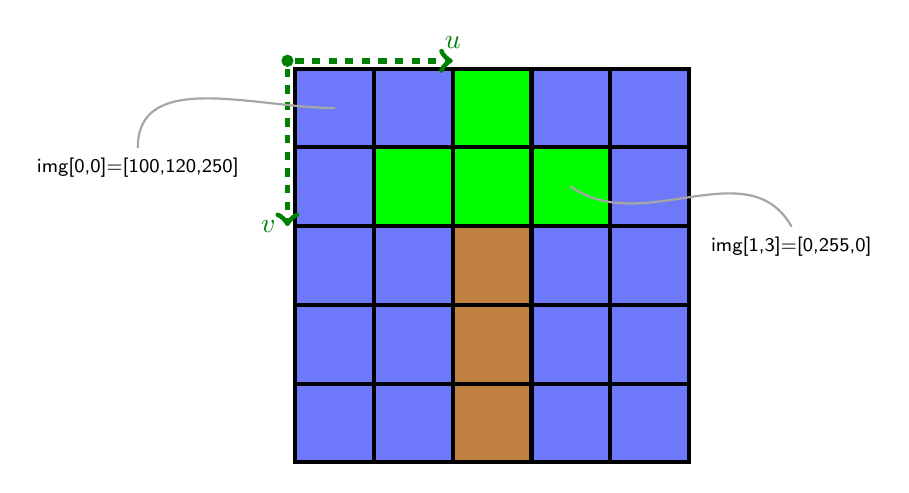
\begin{tikzpicture}  [
    description/.style={draw=gray!70, thick, line cap=round, every node/.style={align=center, font=\scriptsize\sffamily, anchor=north}},
  ]

\definecolor{blue}{RGB}{110,120,250}

\foreach \x in {0,...,4}
    \foreach \y in {0,...,4} 
		%\draw [fill=blue!30!white, line width=1.5] (\x,\y) rectangle (\x+1.0,\y+1.0);
		\draw [fill=blue, line width=1.5] (\x,\y) rectangle (\x+1.0,\y+1.0);
\draw [fill=green, line width=1.5] (2,4) rectangle (3,5);
\draw [fill=green, line width=1.5] (2,3) rectangle (3,4);
\draw [fill=green, line width=1.5] (3,3) rectangle (4,4);
\draw [fill=green, line width=1.5] (1,3) rectangle (2,4);

\draw [fill=brown, line width=1.5] (2,2) rectangle (3,3);
\draw [fill=brown, line width=1.5] (2,1) rectangle (3,2);
\draw [fill=brown, line width=1.5] (2,0) rectangle (3,1);

\draw[dashed, line width=2, ->, color=green!50!black] (-0.1,5) -- (-0.1,3) node[below, left] {$v$};
\draw[dashed, line width=2, ->, color=green!50!black] (0,5.1) -- (2,5.1) node[right, above] {$u$};
\draw[fill, color=green!50!black] (-0.1,5.1) circle (0.07);
\path[description] (3.5,3.5) [out=-35, in=120] to (6.3,3) node {img[1,3]=[0,255,0]};

\path[description] (0.5,4.5) [out=180, in=90] to (-2,4) node {img[0,0]=[100,120,250]};
% ..
\end{tikzpicture}